\documentclass[11pt,a4paper]{article}

\usepackage[T1]{fontenc}
\usepackage[utf8]{inputenc}
\usepackage[italian]{babel}
\usepackage{amsmath,amssymb}
\usepackage[a4paper,margin=2.5cm]{geometry}
\usepackage{array}
\usepackage{siunitx}
\usepackage{booktabs}
\usepackage{graphicx}
\usepackage{float}
\usepackage{hyperref}

\hypersetup{hidelinks}
\setlength{\parindent}{0pt}
\setlength{\parskip}{4pt}
\allowdisplaybreaks
\graphicspath{{figure/}}
\sisetup{output-decimal-marker={,}, group-separator={\,}, per-mode=symbol,
         exponent-product=\cdot, range-phrase={\text{--}}}

\newcommand{\jp}[1]{\left[#1\right]}            % salto [q] = q2 - q1
\newcommand{\av}[1]{\left\langle #1\right\rangle} % media <q> = (q1 + q2)/2
\newcommand{\uma}{u-a}
\newcommand{\upa}{u+a}

\title{Gasdinamica -- Svolgimento esercizio 2\\[2pt]
\large Relazioni di salto per l'energia interna e per l'energia cinetica}
\author{}
\date{Prova del 01/01/1975}

\begin{document}
\maketitle

\section*{Traccia}
Considerare le relazioni di salto per un flusso monodimensionale non stazionario e ricavare da queste le
relazioni di salto per l'energia interna e l'energia cinetica. Esprimere la relazione di salto per l'energia
interna per la variabile dipendente pressione. Mostrare la relazione tra relazione di salto per l'energia
cinetica e quella per la quantità di moto.
\begin{figure}[H]
  \centering
  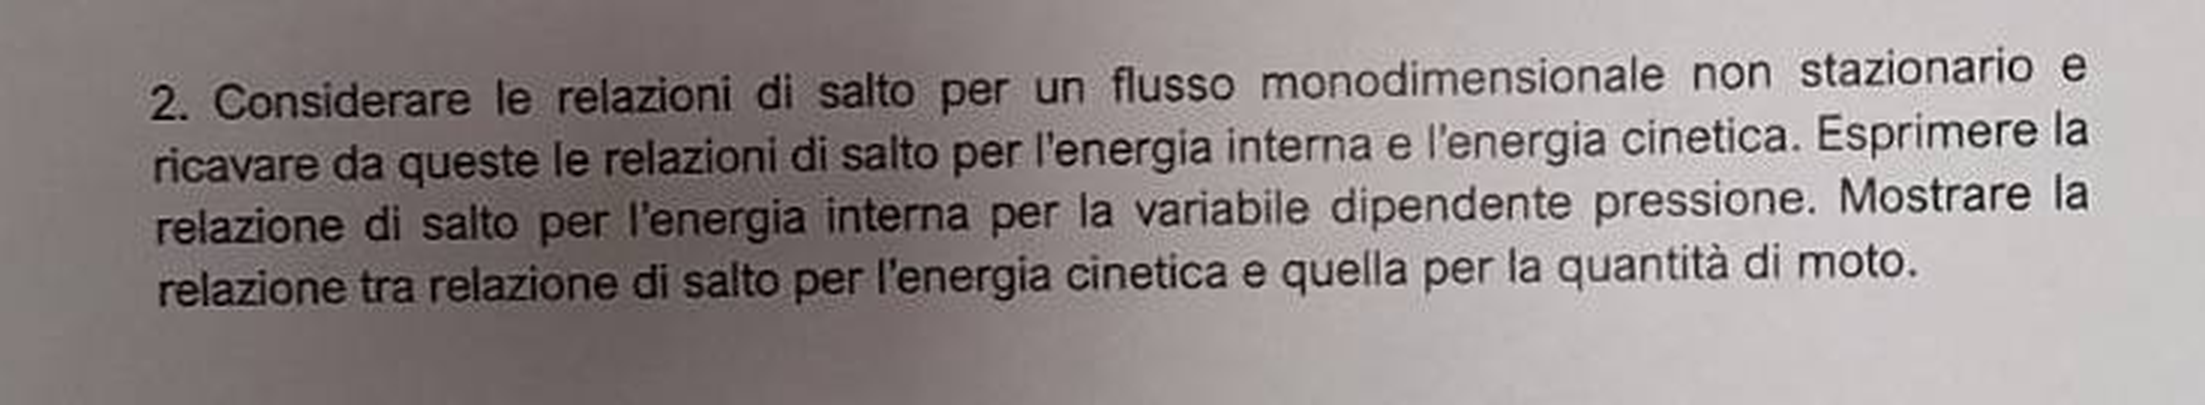
\includegraphics[width=0.9\textwidth]{originale.png}
  \caption{Testo originale dell'esercizio.}
\end{figure}
Tracce affini nel catalogo: B64-E02 (15/06/2021), che chiede di dimostrare che il salto dell'energia cinetica
discende esattamente da quello della quantità di moto e che il salto dell'energia totale si riduce a quello
dell'energia interna; B54-E01 (23/01/2018), bilancio dell'energia cinetica in forma quasi lineare e conservativa
e sua relazione di salto; B32-E01 (10/07/2013), equazione dell'energia cinetica e suo legame con massa e
quantità di moto.

%==============================================================================
\section{Lettura del testo e dati}
Le ``relazioni di salto'' di partenza sono quelle di Rankine--Hugoniot per una discontinuità che si muove con
velocità $w$ in un flusso 1D: massa, quantità di moto, energia totale. Da queste la traccia chiede di ricavare:
\begin{enumerate}
  \item la relazione di salto per l'\textbf{energia cinetica} $u^2/2$;
  \item la relazione di salto per l'\textbf{energia interna} $e_i$;
  \item la stessa relazione con la \textbf{pressione come variabile dipendente}. La interpreto così: come
        l'equazione dell'energia interna $\rho\,De_i/Dt+p\,u_x=0$ si riscrive per il gas perfetto come equazione
        della pressione $p_t+u\,p_x+\gamma p\,u_x=0$, così la relazione di salto per $e_i$ va riscritta con $p$ al
        posto di $e_i$. Ne segue anche la curva di Hugoniot $p_2/p_1$ in funzione di $\rho_2/\rho_1$, che è la
        stessa relazione scritta per le sole grandezze termodinamiche;
  \item il \textbf{legame} fra la relazione per l'energia cinetica e quella per la quantità di moto.
\end{enumerate}
Il problema è letterale. Uso un urto con $M_s=2$ in aria in quiete solo come controllo numerico e per i
diagrammi.

\textbf{Notazione.} Lo stato 1 è a monte (la particella non è ancora stata attraversata dalla discontinuità), lo
stato 2 a valle. Il salto e la media di una grandezza $q$ sono
\[
  \jp{q}=q_2-q_1,\qquad \av{q}=\frac{q_1+q_2}{2}.
\]
Inoltre $v=u-w$ è la velocità relativa alla discontinuità, $m=\rho v$ il flusso di massa che la attraversa,
$\tau=1/\rho$ il volume specifico, $e=e_i+u^2/2$ l'energia totale specifica.

\begin{table}[H]
  \centering
  \begin{tabular}{lll}
    \toprule
    Grandezza & Valore & Note \\
    \midrule
    flusso & 1D non stazionario & discontinuità $x=wt$ \\
    gas & perfetto, $\gamma$ generico & serve solo per la forma in pressione \\
    esempio (controlli, diagrammi) & aria $\gamma=1{,}4$, $M_s=2$ & gas 1 in quiete, $p_1=a_1=1$ \\
    \bottomrule
  \end{tabular}
  \caption{Dati del problema.}
\end{table}

%==============================================================================
\section{Modello e ipotesi}
\begin{itemize}
  \item \textbf{Equazioni di Eulero 1D in forma conservativa}, $U_t+F_x=0$ con $U=(\rho,\rho u,\rho e)$ e
        $F=(\rho u,\rho u^2+p,u(\rho e+p))$: fluido non viscoso, adiabatico, senza forze di volume. Attraverso una
        discontinuità le derivate non esistono e vale solo la forma integrale delle leggi di conservazione:
        per questo il punto di partenza devono essere le grandezze che si \emph{conservano} davvero, cioè massa,
        quantità di moto ed energia totale.
  \item \textbf{Discontinuità a spessore nullo}, rettilinea nel piano $x$--$t$ ($w$ costante) e con stati
        uniformi ai due lati. Le relazioni sono puntuali: se $w$ varia lentamente valgono istante per istante.
        Lo spessore reale dell'urto (pochi liberi cammini medi) è trascurabile rispetto alle scale del flusso.
  \item \textbf{Gas perfetto}, $e_i=p\tau/(\gamma-1)$, solo per la forma in pressione. Le relazioni per
        l'energia cinetica e per l'energia interna valgono per qualunque gas.
\end{itemize}

%==============================================================================
\section{Analisi qualitativa}
Nel continuo le due energie si ottengono dalla quantità di moto e dall'energia totale. Moltiplicando per $u$
l'equazione della quantità di moto, $\rho(u_t+uu_x)+p_x=0$, e usando la continuità:
\[
  \Bigl(\rho\frac{u^2}{2}\Bigr)_t+\Bigl(\rho\frac{u^3}{2}+pu\Bigr)_x=p\,u_x ,\qquad
  (\rho e_i)_t+(\rho e_i u)_x=-p\,u_x ,
\]
dove la seconda è la differenza fra l'energia totale e la prima. Il termine $p\,u_x$, la potenza della pressione
nella compressione o nell'espansione, passa energia dall'una all'altra forma. Quindi \textbf{né l'energia
cinetica né l'energia interna si conservano}: le loro equazioni non sono in forma di divergenza e non si
possono integrare attraverso la discontinuità, perché lì $p$ salta proprio dove $u_x$ è concentrata.

Mi aspetto perciò che:
\begin{itemize}
  \item il salto dell'energia cinetica sia quello della quantità di moto moltiplicato per una velocità
        ``media'', come nel continuo si moltiplica per $u$, e quindi non sia una relazione nuova;
  \item il salto dell'energia interna sia ciò che resta dell'energia totale: il lavoro di compressione
        compiuto da una pressione ``media'';
  \item questa pressione media non coincida con quella che si ha lungo un'isentropica: la relazione per
        l'energia interna attraverso un urto descrive una trasformazione diversa dall'isentropica, e la
        differenza è la produzione di entropia.
\end{itemize}

%==============================================================================
\section{Topologia del campo}
\begin{figure}[H]
  \centering
  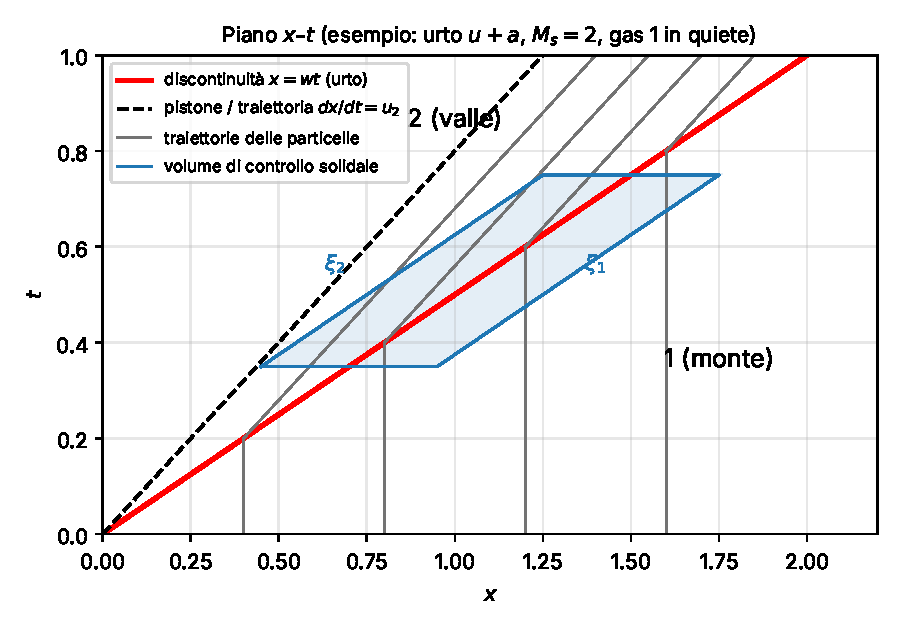
\includegraphics[width=0.66\textwidth]{xt.pdf}
  \caption{Piano $x$--$t$: discontinuità $x=wt$ fra gli stati uniformi 1 (monte) e 2 (valle), traiettorie delle
  particelle e volume di controllo solidale con la discontinuità (esempio: urto $\upa$ con $M_s=2$, generato da un
  pistone impulsivo).}
  \label{fig:xt}
\end{figure}
Nel piano $x$--$t$ (fig.~\ref{fig:xt}) la discontinuità è la retta $x=wt$, fra due stati uniformi. Nell'esempio
è un urto $\upa$: lo stato 1, in quiete, è a destra, e ogni particella, raggiunta dall'urto, passa nello stato 2 e
prende la velocità $u_2$ del pistone. Le traiettorie attraversano la discontinuità ($m\neq0$): è un
\textbf{urto}. Se invece le traiettorie sono parallele alla discontinuità ($w=u$, $m=0$), nessuna particella la
attraversa ed è un \textbf{contatto}: per esso non esistono monte e valle, ma solo un lato 1 e un lato 2.

Il parallelogramma è il volume di controllo $[\xi_2,\xi_1]$ nella variabile $\xi=x-wt$, fermo rispetto alla
discontinuità: è quello su cui si integrano le leggi di conservazione.

%==============================================================================
\section{Bilancio equazioni/incognite}
Le incognite di una discontinuità sono gli stati ai due lati, $(\rho,u,p)_{1,2}$, e la velocità $w$: sette in
tutto. Le relazioni indipendenti sono tre (massa, quantità di moto, energia totale). Noto lo stato 1, basta un
dato in più ($w$, oppure $u_2$, oppure $p_2$) per chiudere il problema. Le relazioni per l'energia cinetica,
per l'energia interna e per la pressione che ricavo sotto sono \textbf{combinazioni} delle tre, non informazioni
nuove. Aggiungere ``la conservazione dell'energia cinetica'' come quarta equazione indipendente sovradeterminerebbe
il problema e sarebbe sbagliato, perché l'energia cinetica non si conserva.

%==============================================================================
\section{Scorciatoie fisiche}
Il salto di un prodotto si scrive \textbf{esattamente} con le medie aritmetiche:
\[
  \jp{ab}=a_2b_2-a_1b_1=\frac{a_1+a_2}{2}(b_2-b_1)+\frac{b_1+b_2}{2}(a_2-a_1)
  =\av{a}\jp{b}+\av{b}\jp{a},
  \qquad
  \jp{\tfrac{a^2}{2}}=\av{a}\jp{a}.
\]
È la versione discreta della regola di derivazione del prodotto, ed è la stessa identità che si usa per
mostrare che attraverso un contatto $\jp{u}=0$. Quindi ogni manipolazione delle equazioni differenziali ha un
equivalente esatto per i salti, con le medie al posto dei coefficienti: le relazioni di salto derivate
\emph{somigliano} alle equazioni quasi lineari, con $\av{u}$, $\av{p}$ al posto di $u$, $p$. Inoltre $w$ è lo
stesso ai due lati, quindi $\jp{v}=\jp{u}$.

%==============================================================================
\section{Calcolo}
\subsection{Relazioni di salto di partenza}
Nella variabile $\xi=x-wt$, solidale con la discontinuità, $U_t+F_x=0$ diventa $U_t+(vU+P)_\xi=0$, con
$P=(0,p,pu)$, perché $F=uU+P$. Integrando sul volume di controllo della fig.~\ref{fig:xt}, gli stati sono
uniformi e il contenuto non cambia nel tempo, quindi il flusso entrante è uguale a quello uscente:
$\jp{vU+P}=0$, cioè $w\jp{U}=\jp{F}$. Per componenti:
\[
  \text{(M)}\ \ \jp{\rho v}=0\ \Rightarrow\ m=\rho_1v_1=\rho_2v_2,\qquad
  \text{(Q)}\ \ m\jp{u}+\jp{p}=0,\qquad
  \text{(E)}\ \ m\jp{e}+\jp{pu}=0 .
\]
(Q) ed (E) seguono da $\jp{\rho uv+p}$ e $\jp{\rho ev+pu}$ portando fuori dal salto la costante $m$.

\subsection{Energia cinetica e legame con la quantità di moto}
Dalla scorciatoia $\jp{u^2/2}=\av{u}\jp{u}$, quindi moltiplicando (Q) per $\av{u}$:
\[
  \boxed{\ \text{(K)}\qquad m\,\Bigl[\frac{u^2}{2}\Bigr]+\av{u}\jp{p}=0
  \quad\Longleftrightarrow\quad
  m\,\Bigl[\frac{u^2}{2}\Bigr]=\av{u}\,m\jp{u}\ }
\]
\textbf{La relazione per l'energia cinetica è quella della quantità di moto moltiplicata per la velocità media}
$\av{u}$, come nel continuo l'equazione dell'energia cinetica è quella della quantità di moto moltiplicata per
$u$. Non è una relazione indipendente: è conseguenza esatta di (M) e (Q).

Usando $m=\rho(u-w)$ (costante) e $\jp{pu}=\av{u}\jp{p}+\av{p}\jp{u}$, la stessa relazione si scrive come un
bilancio con sorgente:
\[
  -w\Bigl[\rho\frac{u^2}{2}\Bigr]+\Bigl[\rho\frac{u^3}{2}+pu\Bigr]=\av{p}\jp{u},
\]
immagine esatta dell'equazione $(\rho u^2/2)_t+(\rho u^3/2+pu)_x=p\,u_x$, con $\partial_t\to-w\jp{\cdot}$,
$\partial_x\to\jp{\cdot}$ e il termine non conservativo $p\,u_x\to\av{p}\jp{u}$. Il secondo membro non è nullo:
attraverso un urto l'energia cinetica non si conserva.

L'energia cinetica dipende dall'osservatore. Nel riferimento della discontinuità la stessa costruzione dà
$m\jp{v^2/2}+\av{v}\jp{p}=0$. Con $\av{v}=\av{u}-w$ la differenza con (K) è $-w\,(m\jp{u}+\jp{p})$, cioè $-w$
volte la (Q): il cambio di riferimento è assorbito ancora dalla quantità di moto.

\subsection{Energia interna}
Sottraggo (K) da (E), con $\jp{e}=\jp{e_i}+\jp{u^2/2}$ e $\jp{pu}=\av{u}\jp{p}+\av{p}\jp{u}$; il termine
$\av{u}\jp{p}$ si elide:
\[
  \boxed{\ \text{(I)}\qquad m\jp{e_i}+\av{p}\jp{u}=0\ }
  \qquad\Longleftrightarrow\qquad
  -w\jp{\rho e_i}+\jp{\rho e_iu}=-\av{p}\jp{u},
\]
immagine di $(\rho e_i)_t+(\rho e_iu)_x=-p\,u_x$. Il salto dell'energia totale si riduce quindi a quello
dell'energia interna: noti (M) e (Q), le relazioni (E) e (I) sono equivalenti.

Per un urto ($m\neq0$) uso $v=m\tau$, quindi $\jp{u}=\jp{v}=m\jp{\tau}$, e divido per $m$:
\[
  \boxed{\ \jp{e_i}+\av{p}\jp{\tau}=0\quad\Longleftrightarrow\quad
  e_{i2}-e_{i1}=\frac{p_1+p_2}{2}\,(\tau_1-\tau_2)\ }
\]
È l'\textbf{equazione di Hugoniot}: contiene solo grandezze termodinamiche, quindi vale in ogni riferimento e per
qualunque gas. Ha la forma del primo principio per una trasformazione adiabatica reversibile,
$de_i=-p\,d\tau$, ma con la \textbf{pressione media} $\av{p}$ al posto di $p$: l'energia interna cresce del
lavoro di compressione compiuto dalla media delle pressioni ai due lati.

Allo stesso modo da (Q) si ha $\jp{p}=-m^2\jp{\tau}$: nel piano $p$--$\tau$ gli stati 1 e 2 stanno su una retta di
pendenza $-m^2$ (retta di Rayleigh).

\subsection{Energia interna con la pressione come variabile dipendente}
Per il gas perfetto $e_i=p\tau/(\gamma-1)$, quindi $m\,e_i=pv/(\gamma-1)$ e, essendo $m$ costante,
$m\jp{e_i}=\jp{pv}/(\gamma-1)$. In (I), con $\jp{pv}=\av{p}\jp{v}+\av{v}\jp{p}$ e $\jp{v}=\jp{u}$:
\[
  \frac{\av{v}\jp{p}+\av{p}\jp{u}}{\gamma-1}+\av{p}\jp{u}=0
  \quad\Longrightarrow\quad
  \av{v}\jp{p}+\gamma\av{p}\jp{u}=0 .
\]
Con $\av{v}=\av{u}-w$:
\[
  \boxed{\ \text{(P)}\qquad -w\jp{p}+\av{u}\jp{p}+\gamma\av{p}\jp{u}=0\ }
\]
È l'immagine esatta dell'equazione della pressione $p_t+u\,p_x+\gamma p\,u_x=0$, con i coefficienti $u$ e $p$
sostituiti dalle loro medie. Vale anche per il contatto.

Per un urto, con $\jp{u}=m\jp{\tau}$ e $\av{v}=m\av{\tau}$, dividendo per $m$:
\[
  \av{\tau}\jp{p}+\gamma\av{p}\jp{\tau}=0 ,
\]
che ha la forma della \textbf{isentropica} $\tau\,dp+\gamma p\,d\tau=0$, ancora con le medie. Risolvendo per la
pressione, con $r=\rho_2/\rho_1=\tau_1/\tau_2$:
\[
  \frac{p_2}{p_1}=\frac{(\gamma+1)\,r-(\gamma-1)}{(\gamma+1)-(\gamma-1)\,r},
  \qquad r\to\frac{\gamma+1}{\gamma-1}\ \text{per}\ \frac{p_2}{p_1}\to\infty ,
\]
che è la curva di Hugoniot: il rapporto delle densità attraverso un urto è limitato ($r<6$ per l'aria), quello
delle pressioni no.

\subsection{Contatto ($m=0$)}
Da (Q) $\jp{p}=0$; da (I), con $m=0$ e $\av{p}>0$, $\jp{u}=0$; la (K) diventa un'identità. Il salto
dell'energia interna resta libero (moltiplica $m=0$): densità, temperatura ed entropia possono saltare, pressione
e velocità no.

\subsection{Controllo sull'esempio}
Urto $\upa$ con $M_s=2$ in aria in quiete, $p_1=a_1=1$, $\rho_1=1{,}4$: dalle relazioni di Rankine--Hugoniot
\begin{gather*}
  w=M_sa_1=2,\qquad \frac{p_2}{p_1}=1+\frac{2\gamma}{\gamma+1}(M_s^2-1)=4{,}5,\\
  \frac{\rho_2}{\rho_1}=\frac{\gamma+1}{\gamma-1+2/M_s^2}\approx2{,}67,\qquad
  u_2=w\Bigl(1-\frac{\rho_1}{\rho_2}\Bigr)=1{,}25,
\end{gather*}
quindi $m=-\rho_1w=-2{,}8$, $\av{u}=0{,}625$, $\av{p}=2{,}75$. Allora:
\begin{itemize}
  \item (K): $m\jp{u^2/2}=-2{,}19$ e $\av{u}\jp{p}=2{,}19$;
  \item (I): $m\jp{e_i}=-3{,}44$ e $\av{p}\jp{u}=3{,}44$;
  \item (P): $-w\jp{p}=-7$, $\av{u}\jp{p}=2{,}19$, $\gamma\av{p}\jp{u}=4{,}81$, con somma nulla;
  \item Hugoniot: con $r\approx2{,}67$ la formula dà $p_2/p_1=4{,}5$.
\end{itemize}
Il lavoro del pistone per unità di area e di tempo, $p_2u_2=\jp{pu}=5{,}63$, si divide in $\av{u}\jp{p}=2{,}19$,
che va in energia cinetica, e $\av{p}\jp{u}=3{,}44$, che va in energia interna.

%==============================================================================
\section{Verifiche a posteriori}
\begin{itemize}
  \item Esempio $M_s=2$: (K), (I), (P), Hugoniot e Rayleigh sono soddisfatte: verificata.
  \item Limite di salto piccolo: per $\jp{\cdot}\to0$ le medie tendono ai valori locali, e (K), (I), (P)
        tornano le equazioni quasi lineari dell'energia cinetica, dell'energia interna e della pressione:
        verificata.
  \item Contatto: $\jp{p}=\jp{u}=0$ con $\jp{\rho}$ ed $\jp{e_i}$ liberi, come nella teoria del corso:
        verificata.
  \item Invarianza galileiana: sommando $0{,}7$ a tutte le velocità dell'esempio, $\jp{u^2/2}$ passa da $0{,}78$
        a $1{,}66$ ma (K) resta soddisfatta, mentre $\jp{e_i}=1{,}23$ non cambia: verificata.
  \item Hugoniot e isentropica hanno la stessa tangente e la stessa curvatura in 1: per $M_s=1{,}1$ danno
        $p_2/p_1=1{,}245$ e $1{,}244$; per $M_s=2$, $4{,}5$ e $3{,}95$: verificata.
  \item Secondo principio: sul ramo di compressione ($\jp{\tau}<0$) $\jp{e_i}=-\av{p}\jp{\tau}>0$ e la Hugoniot
        sta sopra l'isentropica, quindi $\Delta s>0$; il ramo di espansione sta sotto l'isentropica
        ($\Delta s<0$) ed è escluso: verificata.
  \item Urto forte: $\rho_2/\rho_1\to(\gamma+1)/(\gamma-1)=6$; per $M_s=20$ si ha già $5{,}93$: verificata.
\end{itemize}

%==============================================================================
\section{Risultati}
\begin{table}[H]
  \centering
  \small
  \begin{tabular}{lll}
    \toprule
    Relazione & Forma & Analogo continuo \\
    \midrule
    massa (M) & $\jp{\rho v}=0$, $m=\rho v$ & $\rho_t+(\rho u)_x=0$ \\
    quantità di moto (Q) & $m\jp{u}+\jp{p}=0$ & $\rho\,Du/Dt+p_x=0$ \\
    energia totale (E) & $m\jp{e}+\jp{pu}=0$ & $(\rho e)_t+[u(\rho e+p)]_x=0$ \\
    \midrule
    energia cinetica (K) & $m\jp{u^2/2}+\av{u}\jp{p}=0$ & $\rho\,D(u^2/2)/Dt+u\,p_x=0$ \\
    legame (K)--(Q) & (K) $=\av{u}\times$(Q) & $u\times$ quantità di moto \\
    energia interna (I) & $m\jp{e_i}+\av{p}\jp{u}=0$ & $\rho\,De_i/Dt+p\,u_x=0$ \\
    Hugoniot ($m\neq0$) & $\jp{e_i}+\av{p}\jp{\tau}=0$ & $de_i+p\,d\tau=0$ \\
    pressione (P) & $-w\jp{p}+\av{u}\jp{p}+\gamma\av{p}\jp{u}=0$ & $p_t+up_x+\gamma pu_x=0$ \\
    Hugoniot in $p$ & $\av{\tau}\jp{p}+\gamma\av{p}\jp{\tau}=0$ & $\tau\,dp+\gamma p\,d\tau=0$ \\
    \bottomrule
  \end{tabular}
  \caption{Relazioni di salto (tutte esatte) e loro analogo nel continuo.}
\end{table}
Esplicitamente: $p_2/p_1=[(\gamma+1)r-(\gamma-1)]/[(\gamma+1)-(\gamma-1)r]$, con $r=\rho_2/\rho_1$.

%==============================================================================
\section{Rappresentazioni}
\begin{figure}[H]
  \centering
  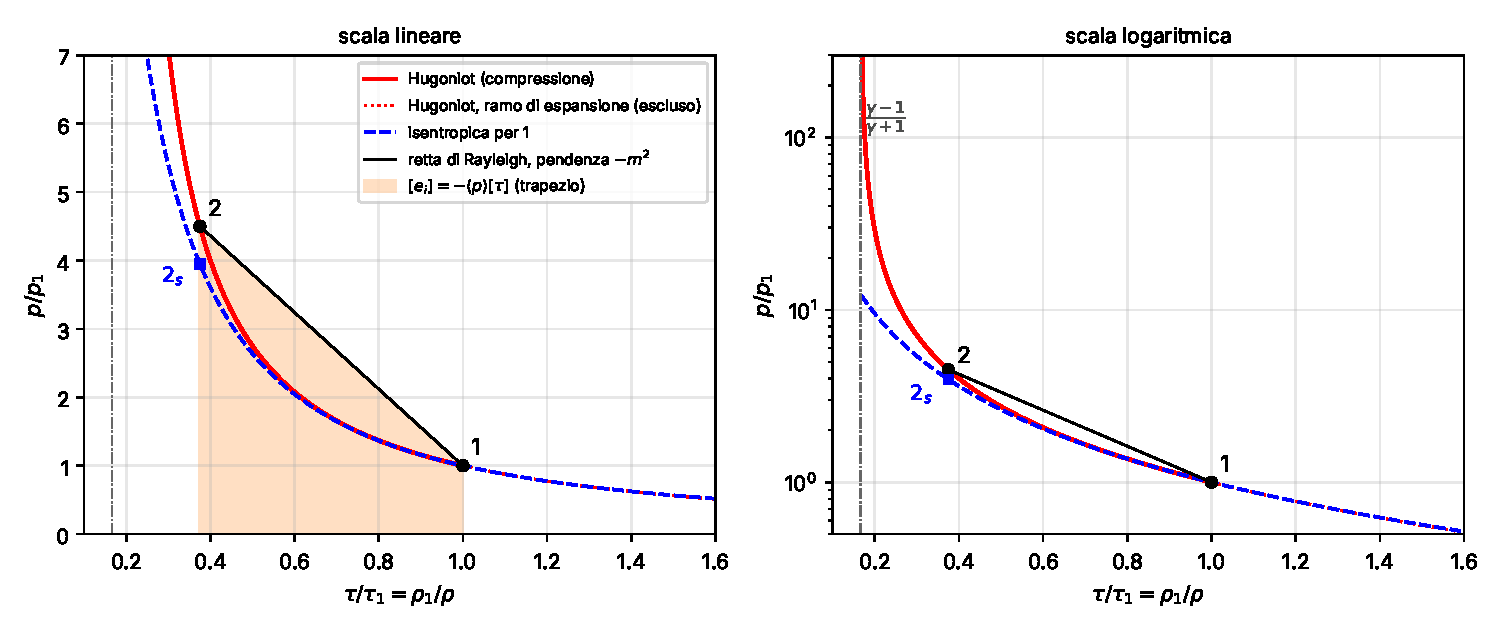
\includegraphics[width=\textwidth]{p_tau.pdf}
  \caption{Piano $p$--$\tau$ per $\gamma=1{,}4$: curva di Hugoniot per lo stato 1, isentropica per 1, retta di
  Rayleigh e stato 2 dell'esempio $M_s=2$; $2_s$ è lo stato isentropico alla stessa densità. A sinistra, scala
  lineare con l'area $\jp{e_i}$; a destra, scala logaritmica fino all'asintoto $\tau/\tau_1=(\gamma-1)/(\gamma+1)$.}
  \label{fig:ptau}
\end{figure}
Nella fig.~\ref{fig:ptau} a sinistra (scala lineare) l'area arancione è il trapezio sotto la retta di Rayleigh
fra $\tau_2$ e $\tau_1$, cioè $\av{p}(\tau_1-\tau_2)=\jp{e_i}$: è la forma grafica dell'equazione di Hugoniot.
Una compressione isentropica fino alla stessa densità richiede solo l'area sotto la curva tratteggiata, più
piccola, e arriva in $2_s$, a pressione minore. Nell'esempio ($p_1=1$, $\rho_1=1{,}4$) $\jp{e_i}=1{,}23$ contro
$0{,}86$ dell'isentropica. Vicino a 1 le due curve
sono indistinguibili. A destra, in scala logaritmica, si vede tutto il ramo di compressione: la Hugoniot sale
verticalmente verso l'asintoto $\tau_2/\tau_1=1/6$, mentre l'isentropica prosegue fino a $\tau\to0$. Il ramo di
espansione della Hugoniot ($\tau>\tau_1$, puntinato) è appena sotto l'isentropica.

\begin{figure}[H]
  \centering
  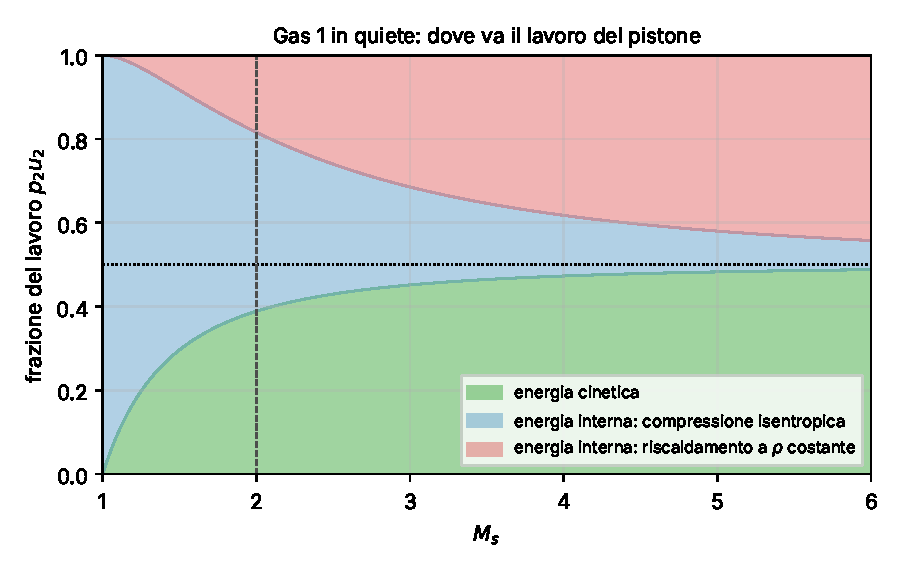
\includegraphics[width=0.66\textwidth]{ripartizione.pdf}
  \caption{Gas 1 in quiete: ripartizione del lavoro del pistone $p_2u_2$ fra energia cinetica, compressione
  isentropica fino a $\rho_2$ e riscaldamento a densità costante, in funzione di $M_s$.}
  \label{fig:rip}
\end{figure}
La fig.~\ref{fig:rip} traduce (K) e (I) in una ripartizione di energia. Per il gas in quiete $\av{u}=u_2/2$, quindi
la frazione che va in energia cinetica è $\av{u}\jp{p}/(p_2u_2)=(p_2-p_1)/(2p_2)$ e quella in energia interna è
$(p_1+p_2)/(2p_2)$. Per $M_s=2$ (linea tratteggiata) le frazioni sono $39\%$ in energia cinetica, $43\%$ in
compressione isentropica e $18\%$ in riscaldamento. Al crescere di $M_s$ la cinetica tende a metà del lavoro
(linea puntinata) e quasi tutta l'energia interna diventa riscaldamento.

%==============================================================================
\section{Discussione fisica}
\textbf{Perché la media aritmetica.} Le medie non sono un'approssimazione: escono dall'identità
$\jp{ab}=\av{a}\jp{b}+\av{b}\jp{a}$, che è esatta. Moltiplicare (Q) per $\av{u}$ dà esattamente il salto
dell'energia cinetica; moltiplicarla per $u_1$ o per $u_2$ no. Il termine di scambio $p\,u_x$, che non ha senso
dove $p$ salta e $u_x$ è concentrata, attraverso la discontinuità ``vale'' $\av{p}\jp{u}$: questo valore è fissato
dalle tre leggi di conservazione, non dalla struttura interna dell'urto.

\textbf{Dove nasce l'entropia.} Nel continuo $de_i=-p\,d\tau$ è l'isentropica, $\tau\,dp+\gamma p\,d\tau=0$. Le
relazioni di salto sono le stesse con $p$ e $\tau$ sostituiti dalle medie ai due estremi: è la regola dei
trapezi applicata all'isentropica. Il primo principio vale ancora, ma il lavoro di compressione è quello della
media delle pressioni, maggiore di quello lungo l'isentropica, perché l'isentropica nel piano $p$--$\tau$ è convessa.
L'eccesso, il trapezio meno l'area sotto l'isentropica, è energia dissipata dentro lo spessore dell'urto dalla
viscosità e dalla conduzione, che il modello non vede ma il cui effetto netto è fissato dalle relazioni di salto.
L'errore della regola dei trapezi è del terzo ordine nell'ampiezza: quindi $\Delta s\propto\jp{p}^3$. È per questo
che gli urti deboli si possono trattare come onde isentropiche.

\textbf{Dove va il lavoro.} Per un urto generato da un pistone, $\jp{e_i}/\jp{u^2/2}=(p_1+p_2)/(p_2-p_1)$. Negli
urti deboli quasi tutto il lavoro va in energia interna, ma in modo quasi reversibile: è un'onda acustica, e
l'energia cinetica è del secondo ordine. Negli urti forti c'è equipartizione: metà del lavoro va in energia cinetica
e metà in energia interna, e quest'ultima è quasi tutta dissipata (fig.~\ref{fig:rip}).

\textbf{Che cosa è invariante.} L'energia interna, la pressione e l'Hugoniot dipendono solo da $\jp{u}=\jp{v}$ e
dalla termodinamica, quindi non dipendono dal riferimento. L'energia cinetica sì, e la differenza fra due
riferimenti è un multiplo della quantità di moto. Nel riferimento dell'urto, (I) più la (K) relativa danno
$\jp{h+v^2/2}=0$: l'urto, che lì è stazionario, conserva l'entalpia totale relativa.

\textbf{Conseguenza pratica.} La forma conservativa da usare attraverso un urto è quella dell'energia
\emph{totale}. Un modello che conservasse l'energia cinetica, o che integrasse l'equazione della pressione
$p_t+up_x+\gamma pu_x=0$ senza i coefficienti medi giusti, darebbe salti isentropici, e quindi urti con
velocità e stati sbagliati.

\end{document}
